\documentclass{article}
\usepackage{graphicx}
\graphicspath{ {images/} }


\newcommand{\tab}[1]{\hspace{.1\textwidth}\rlap{#1}}

\begin{document}
	
\begin{titlepage}
	\newcommand{\HRule}{\rule{\linewidth}{0.5mm}} % Defines a new command for the horizontal lines, change thickness here

	\center % Center everything on the page
	 
	%----------------------------------------------------------------------------------------
	%	LOGO SECTIONS
	%----------------------------------------------------------------------------------------

	
\includegraphics[width=\textwidth]{front-page}

	%----------------------------------------------------------------------------------------
	%	TITLE SECTION
	%----------------------------------------------------------------------------------------

	\HRule \\[0.4cm]
	{ \huge \bfseries Software Requirements Specification
	and
	Technology Neutral Process Design}\\[0.4cm] % Title of your document
	\HRule \\[1.5cm]
	 
	%----------------------------------------------------------------------------------------
	%	MEMBERS, TEAM NAME SECTION
	%----------------------------------------------------------------------------------------

	\begin{minipage}{0.5\textwidth}
	\begin{flushleft} \large
	\emph{Members:}\\% add your name
	Matthew Botha 14214742

	Gershom Maluleke 13229908


	Nathan Dunkley 14145759

	Aiden Malan

	Sello Thosago

	Nsovo Baloyi 12163262

	Matheu Botha 14284104
	\end{flushleft}
	\end{minipage}
	~
	\begin{minipage}{0.4\textwidth}
	\begin{flushright} \large
	{ \huge \bfseries Team India }% Title of document
	{\large \today}\\
	{\large v0.1}
	\end{flushright}
	\end{minipage}\\[4cm]
\end{titlepage}


	\newpage
	
	\section{Introduction}
	
	The purpose of this document is to outline the core functionality of the new computer science publication system in a technology neutral design specification. This design is not necessarily a depiction of what the final system will look like. During the development of the system it is possible that new functionalities are added, or old ones removed. This is merely the first iteration of the development cycle. Which can be revised in the future. As well as iterativly enhanced and detailed as the need arises. 

	\section{Vision}

	This projects aim is to provide a system to facilitate the administration of postgraduate publications, including but not limited to journal articles and conference papers. It should be able to store information on Users, Authors and Publications as well as employ a authentication system to ensure only specified parties within the system have access to operations on the stored information.
	The purpose of keeping track of the publications is, in part, to keep track of the DoE and UP weighted units earned by Users and/or authors. The reason for this is that these users/authors are required to publish a certain amount of units each year in order to determine pay, research funding, and maintaining their research position.

	\section{Background}
	Currently the publications are kept track of with a complicated excel spreadsheet. The purpose of the spreadsheet is to keep track of the status of publications in order to generate a report detailing the units earned by a researcher. There are many drawbacks to this system. It is tedious to maintain the spreedsheet. Data is spread over multiple sheets. The larger the database gets the slower it preforms. The information is displayed in a raw textual format which makes it a daunting task to sit through and analyse. It is difficult to add new functionality and change or enhance existing functionality. When pulling in data from multiple sheets it becomes difficult to debug the Lookups.

	\section{Software Architecture Documentation}

		\subsection{Architecture requirements}
			\subsubsection{Architectural scope}

			\subsubsection{Quality requirements}
					\begin{itemize}
					  \item Reliability - The reports generated from the data provided to the system should be
					  \item Scalability - It is estimated that there will be approximatly one hundred users. The system should be able to handle each user being active at the same time even though it is unlikly.
					  \item Cost - Generating a report for all data in the system will be the worst case scenario in this system and thus have a high cost. The system should however be able to produce subsets of the report at a relativly low cost. For example a report for all researchers under a specific research group.
					  \item Security - There should be strict access right applied to each of the subsystems and their components. This means that if a user, by definition of the buisness rules, is not allowed to access a certain functionality, then they will be denied access.
					  \item Auditability - Actions performed on the system should be logged in a manner that would allow one to trace back the history of actions performed on the system.
					\end{itemize}

			\subsubsection{Integration and access channel requirements}
				The system will operate in a standalone fashion. In the future, however, it may require intergration with google calender.
				This service should be accessable via web based clients. i.e. web based clients,mobile browsers. As well as an Android application.

			\subsubsection{Architectural constraints}
				Client has not provided any architecture constraints.
				
	%----------------------------------------------------------------------------------------
	%	Architectural patterns or styles
	%----------------------------------------------------------------------------------------

		\subsection{Architectural patterns or styles}
	

		\subsection{Architectural patterns or styles}
		On this section we will be describing the different patterns and styles to be used when developing the CS 		        Research System.
		\setcounter{secnumdepth}{5}
		\subsubsection{Client-server pattern} % level 1
		\begin{itemize}
		 \item Segregates the system into two applications, where the client makes requests to the server. In many 				cases, the server is a database with application logic represented as stored procedures.
		

         \item  The main reason why we chose this pattern is because sensitive and personal data pertaining to the 				name, emails and other client information must be kept secure. Client/Server architecture provides a far 			higher 	degree of security and data integrity. The nature of the CS Report System necessitates a means of 				centralised data access and a system featuring high maintainability. The Client/Server architecture ensures that changes 	made to the system are immediately visible to all clients.
         \end{itemize}
         \paragraph{Server} % level 2
         \begin{itemize}
          \item The Server handles storage of data into the database and provides data on request. The Server is responsible for all back end functions of the software including the verification 	of users for security.
         
           \end{itemize}
            \paragraph{Client} % level 3
         \begin{itemize}
          \item The client is responsible for the front end of the CS report system. It also allows users to 	send 			queries to the server and requesting for various services offered by the server. The 	client also provides 			an interface between the system  and its users.  	
           \end{itemize}
           
           \subsubsection{Authentication Enforcer pattern} % level 1
           
			 \begin{itemize}
          \item  The Authentication Enforcer pattern handles the authentication logic across all of the actions 						within the Web tier. It assumes responsibility for authentication and verification of user identity and 					delegates direct interaction with the security provider to a helper class. This applies not only to 						password-based authentication, but also to client certificate-based authentication and other 								authentication schemes that provide a user’s identity, such as Kerberos. 
        	\item This pattern will help us improve security of the system while keeping the scalability and 						performance well maintained since the Authentication Enforcer pattern provides a consistent and structured way to handle authentication and verification of requests across actions within Web-tier components and also 		supports MVC architecture without duplicating the code.	
           \end{itemize}           
           
            \subsubsection{Dependency Injection} % level 1
            
             \begin{itemize}
          \item  Dependency injection implements inversion of control for software libraries. The design pattern 					allows a client to remove all knowledge of a concrete implementation that it needs to use. This helps 					isolate the client from the impact of design changes and defects. It promotes re-usability, testability 					and maintainability
        	\item The benefits of using Dependency Injection in our system, is that it will ensure loose coupling of 				code between the different modules that need to be implemented. Decoupling of code will ensure that the 					code in the system are cleaner, easier to modify when required and easier to adapt and implement for reuse.	
           \end{itemize} 
           
           
           \subsubsection{Blackboard pattern} % level 1
            
             \begin{itemize}
          \item  The blackboard pattern allows multiple processes to work closer together on separate threads, 						polling and reacting if needed. The CS Report System will be separated through layers. There will be User 			Interface layer, services layer and process layer which will include Business logic and data.  User	 					Interface layer will handle interaction like receiving input like login credentials from users. The 						service layer will handle services like opening a research group and deleting a research group and lastly 			process layer will process services rendered for authorization. Separation through layers will enhance 					performance, how the software reacts,  manageability and reusability.
        	
           \end{itemize} 
           
         
           
           \subsubsection{MVC} % level 1
            \begin{itemize}
          \item  Model View Controller divides the web portion of the server into three interconnected parts, so as 					to 	separate internal representations of information from the ways that information is presented to or 					accepted from the user. This ensures reusability  of code, easy to maintain code and an added maintenance 			benefit as well as ensure separation of concerns, cohesion, decoupling of components and pluggability on 					the CS 	Report System.
			\end{itemize}         	
        	
         
            \paragraph{Model} % level 2
            \begin{itemize}
            \item The Model directly manages manages the data on the database and the overall flow of the software.
            \end{itemize} 
            \paragraph{View} % level 3
              \begin{itemize}
            \item Data can be represented and structured sufficiently using HTML.
            \end{itemize} 
            \paragraph{Controller} % level 4
              \begin{itemize}
            \item The controller will accept the input from the user and convert it into commands that 		the 					model or view can understand.
            
              \end{itemize} 		
		

		\subsection{Architectural tactics or strategies}

		\subsection{Use of reference architectures and frameworks}

		\subsection{Access and integration channels}
			\subsubsection{Access Channels}
				The user will be able to access the system, provided they are logged in, via the web either with a PC or a smartphone.
				It is important that the system has a user friendly interface, especially for mobile devices, to make it as easy to use as possible.
				The user will also be able to use the system via an Android application if they so choose.
			\subsubsection{Integration Channels}
				The system will integrate with external systems via a MySQL database.

		\subsection{Technologies}
		When designing a system the consideration of technologies or platforms, that will be used, is of great importance. This section will describe the technologies that will be used for the CS report system, as well as give reasons for the choices made. The CS report system will bring together several technologies to make one working system. Since the system will include two facets, the web interface and the mobile interface, the choice of technologies is important. Regardless of the technologies chosen the system must remain must remain efficient and functional on both interfaces. The technologies that will be used include and not limited to:
		
		 \textbf{Database:}\par
		 \begin{itemize}
		\item  \textbf{MongoDB} is a cross platform document-oriented database. This database, because it is a NoSQL database. NoSQL over the traditional SQL relational database for its speed when accessing data. MongoDB also stores its data in a similar format to JSON which will go well with the other technologies to be mentioned later in the text.
		\end{itemize}
		
		\textbf{Web Interface Technologies:}\par
		\begin{itemize}
		
		\item \textbf{HTML5} is latest version of the standard markup language for displaying information/ webpages using the HTTP or HTTPS protocols on the web. 
\item \textbf{CSS3 together with the Bootstrap framework} for the styling of the webpages. CSS is the standard style sheet language used with HTML. The Bootstrap framework provides preprogramed styles that can be used to our convenience.
\item \textbf{JavaScript}, in particular the AngularJS framework for providing functionality in the webpage. JavaScript is a client-side language and will provide a way for the webpage to communicate with the database and server. AngularJS over jQuery because it provides more functionality and works well with NodeJS and MongoDB.
\item \textbf{NodeJS} for the server-side scripting. It will communicate with the database. It is fast and works well with AngularJS and MongoDB.
\end{itemize}

\textbf{Mobile Interface Technologies:}\par
\begin{itemize}
\item \textbf{Java and XML} will be used for the Android application development. Java and XML are used together to make Android applications.
\item \textbf{Gradle}
\end{itemize}
\textbf{Operating Systems:}\par
\begin{itemize}
\item \textbf{PC Platforms} \par
The system will run on the 3 most widely used platforms namely Linux, MacOS and Windows. It will be supported by Google Chrome, Safari and Mozilla Firefox. The server will run on a Linux platform.
\item \textbf{Mobile Platforms} \par
Android OS will be the focal mobile OS because of its popularity; haven said that, the system can be adapted to run on iOS and Windows Mobile as well.
\end{itemize}
\textbf{Other Technologies to be considered:}\par
\begin{itemize}
\item \textbf{Google Calendar API}. The Google calendar API can be integrated into both the web based and mobile interfaces. This will allow users to enter their schedule e.g. Due date for reports, conference dates
\end{itemize}



		
	
	\section{Functional Requirements and Application Design}
		\subsection{Use case Prioritisation}
			\subsubsection{User Subsystem}
				Register User: Critical\par
				Update User: Important\par
				Login User: Critical\par
				Logout User: Critical\par
				Add to Publication: Important
			\subsubsection{Publication Subsystem}
			\textbf{Create Publication:} Important\\
			\textbf{View Publication:} Nice-to-Have\\
			\textbf{Update Publication:} Important\\
			\textbf{Remove Publication:} Important\\
			\textbf{Add Author:} Important\\
			\textbf{Remove Author:} Important\\
			\subsubsection{Conference Subsystem}
				\textbf{Add Conference:} important\\
				\textbf{Update Conference:} important\\
				\textbf{Delete Conference:} important
			\subsubsection{Journal Subsystem}
				\textbf{Add Journal:} important\\
				\textbf{Update Journal:} important\\
				\textbf{Delete Journal:} important
			\subsubsection{Thesis Subsystem}
				\textbf{Add Thesis:} important\\
				\textbf{Update Thesis:} important\\
				\textbf{Delete Thesis:} important
			\subsubsection{Research and Authors Subsystem}
				\textbf{Create research paper:} important\\
				\textbf{Update research paper:} important\\
				\textbf{Remove research paper:} important\\
				\textbf{View research paper:} nice to have\\
			\subsubsection{Report Subsystem}
				\textbf{Log In to System:} critical\\
				\textbf{View Available Reports:} important\\
				\textbf{Select Filters to Apply to Reports:} important\\
				\textbf{Select Output Type of Report:} nice-to-have\\
				\textbf{Show Report:} important\\
		\subsection{Use case/Services contracts}
			\subsubsection{User Subsystem}
				\paragraph{Pre-conditions:}
				\paragraph{Register user:} The user can not be registered to the system already and the user registering a new user has to be admin.
				\paragraph{Update user:} The user has to be logged in first before they can update their profile and they can only update their own profile.
				\paragraph{Login user:} The user has to be registered to the system first.
				\paragraph{Logout user:} The user has to be logged in first.
				\paragraph{Add to publication:} The user has to be logged in first and the publication has to exist in the system
				\paragraph{Post-conditions:}
				\paragraph{Register user:} The user is now registered and added to the database.
				\paragraph{Update user:} The user's profile is updated and the changes are saved to the database.
				\paragraph{Login user:} The user is logged into the system.
				\paragraph{Logout user:} The user is logged out of the system.
				\paragraph{Add to publication:} The user's name is now added to the author's of the selected publication.
			\subsubsection{Publication Subsystem}
				\textbf{Use Cases:}\\
				\indent \textbf{3.1 Create Publication:}\\
					\indent \indent \textbf{Pre-conditions:}The user must be logged into the system\\
					\indent \indent \textbf{Post-conditions:}The publication is created\\
				\indent \textbf{3.2 View Publication:}\\
					\indent \indent \textbf{Pre-conditions:}The user must be logged onto the system and the publication must be created before hand\\
					\indent \indent \textbf{Post-conditions:}The user will be able to view and edit(Add authors etc.) to the publication.\\
				\indent \textbf{3.3 Update Publication:}\\
					\indent \indent \textbf{Pre-conditions:} The user must be logged onto the system and the publication must be created before hand\\
					\indent \indent \textbf{Post-conditions:}The publication is updated\\
				\indent \textbf{3.4 Remove Publication:}\\
					\indent \indent \textbf{Pre-conditions:}The user must be logged onto the system, the publication must be created before hand and the user must confirm the removal of the publication\\
					\indent \indent \textbf{Post-conditions:}The publication will be removed\\
				\indent \textbf{3.5 Add Author:}\\
					\indent \indent \textbf{Pre-conditions:}The user must be logged onto the system and the publication must be created before hand\\
					\indent \indent \textbf{Post-conditions:}A new author is added to the publication\\
				\indent \textbf{3.6 Remove Author:}\\
					\indent \indent \textbf{Pre-conditions:}The user must be logged onto the system, the publication must be created before hand and the user must confirm the removal of the selected author\\
					\indent \indent \textbf{Post-conditions:}The author is removed from the publication\\
			\subsubsection{Conference Subsystem}
				\textbf{Add Conference:}\\
					\indent \textbf{Pre-conditions:} The user must be logged in.\\
					\indent \textbf{Post-conditions:} The conference is added.\\
				\textbf{Update Conference:}\\
					\indent \textbf{Pre-conditions:} The user must be logged in and a the conference must be added prior to this use case.\\
					\indent \textbf{Post-conditions:} The conference is updated.\\
				\textbf{Delete Conference:}\\
					\indent \textbf{Pre-conditions:} The user must be logged in and a the conference must be added prior to this use case.\\
					\indent \textbf{Post-conditions:} The conference is deleted.\\
			\subsubsection{Journal Subsystem}
				\textbf{Add Journal:}\\
					\indent \textbf{Pre-conditions:} The user must be logged in.\\
					\indent \textbf{Post-conditions:} The journal is added.\\
				\textbf{Update Journal:}\\
					\indent \textbf{Pre-conditions:} The user must be logged in and a the journal must be added prior to this use case.\\
					\indent \textbf{Post-conditions:} The journal is updated.\\
				\textbf{Delete Journal:}\\
					\indent \textbf{Pre-conditions:} The user must be logged in and a the journal must be added prior to this use case.\\
					\indent \textbf{Post-conditions:} The journal is deleted.\\
			\subsubsection{Thesis Subsystem}
				\textbf{Add Thesis:}\\
					\indent \textbf{Pre-conditions:} The user must be logged in.\\
					\indent \textbf{Post-conditions:} The thesis is added.\\
				\textbf{Update Thesis:}\\
					\indent \textbf{Pre-conditions:} The user must be logged in and a the thesis must be added prior to this use case.\\
					\indent \textbf{Post-conditions:} The thesis is updated.\\
				\textbf{Delete Thesis:}\\
					\indent \textbf{Pre-conditions:} The user must be logged in and a the thesis must be added prior to this use case.\\
					\indent \textbf{Post-conditions:} The thesis is deleted.\\
			\subsubsection{Researchers and Authors Subsystem}
				\indent \textbf{3.1 Create Research Paper:}\\
					\indent \indent \textbf{Pre-conditions:}The user must be logged into the system. The user must also be either HOD, research leader or author.\\
					\indent \indent \textbf{Post-conditions:}The research paper is created.\\
					\begin{figure}
						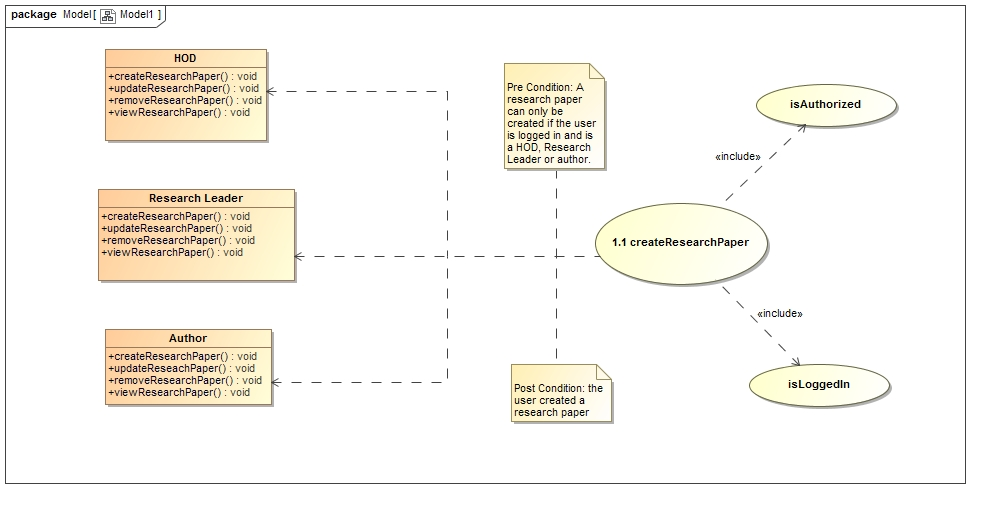
\includegraphics[width=\textwidth]{createResearchPaper}
						\caption{Pre and Post conditions create function}
					\end{figure}
				\indent \textbf{3.2 Update Research Paper:}\\
					\indent \indent \textbf{Pre-conditions:}The user must be logged onto the system and the research paper must exist.\\
					\indent \indent \textbf{Post-conditions:}The user will be able to view and edit(Add authors etc.) to the research paper.\\
					\begin{figure}
						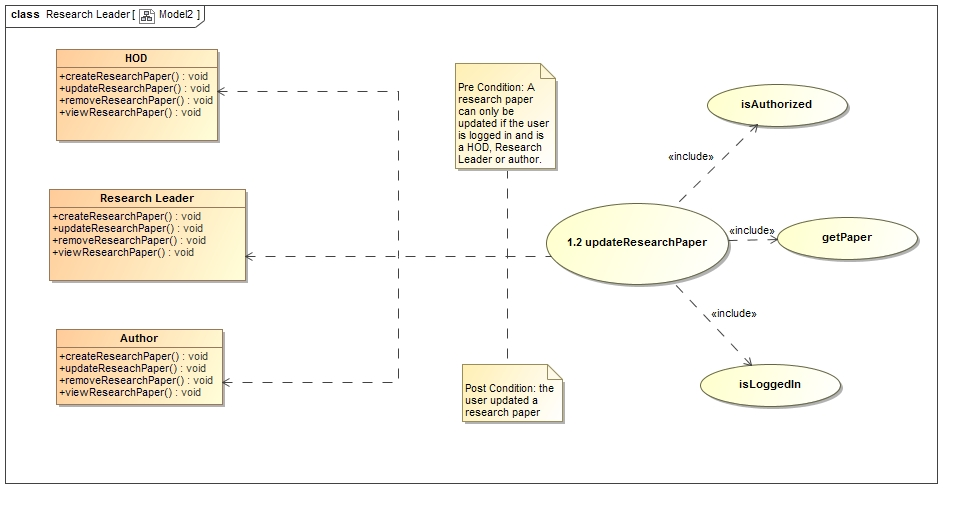
\includegraphics[width=\textwidth]{updatePAper}
						\caption{Pre and Post conditions update function}
					\end{figure}
				\indent \textbf{3.3 Remove Research Paper:}\\
					\indent \indent \textbf{Pre-conditions:} The user must be logged onto the system and the research paper must exist.\\
					\indent \indent \textbf{Post-conditions:}The the research paper is deleted.\\
					\begin{figure}
						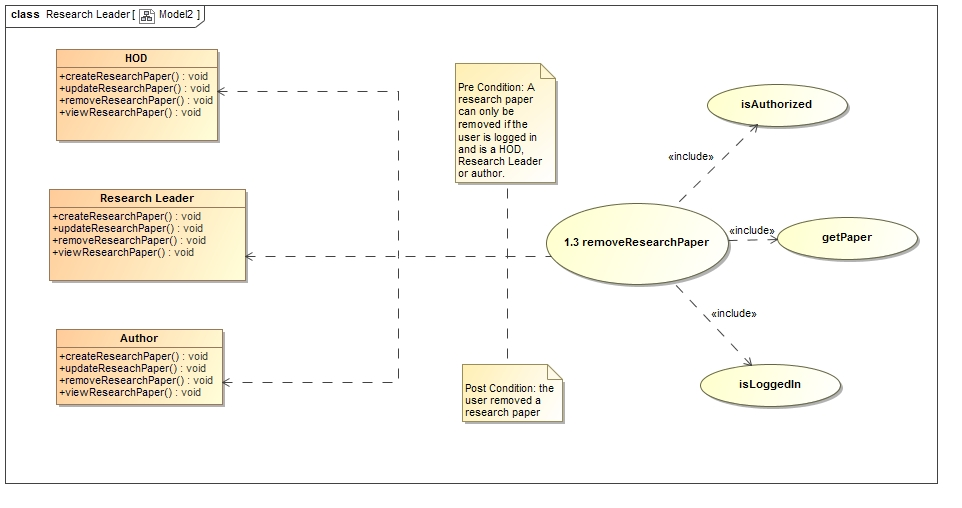
\includegraphics[width=\textwidth]{removeResearch}
						\caption{Pre and Post conditions remove function}
					\end{figure}
				\indent \textbf{3.4 View Research Paper:}\\
					\indent \indent \textbf{Pre-conditions:}The user must be logged onto the system, the research paper must exist.\\
					\indent \indent \textbf{Post-conditions:}The publication can be viewed\\
					\begin{figure}
						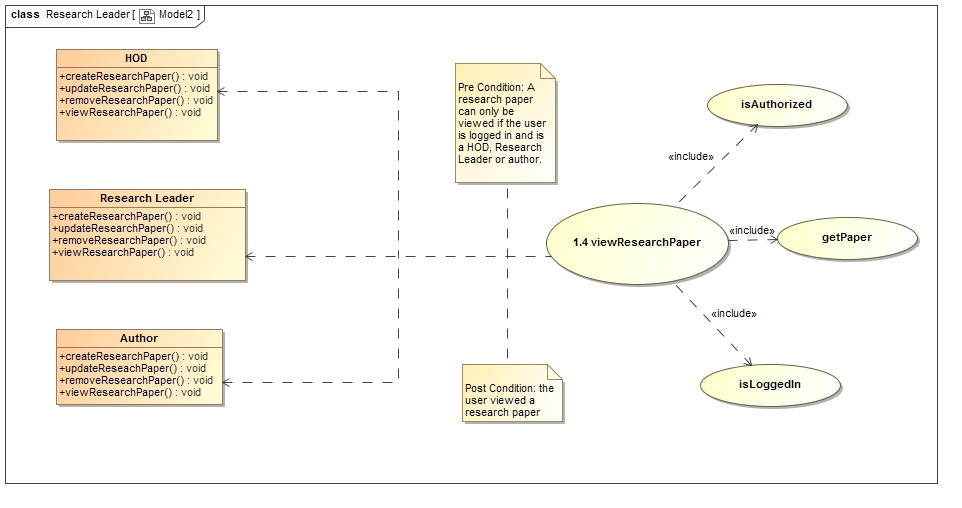
\includegraphics[width=\textwidth]{viewPaper}
						\caption{Pre and Post conditions view function}
					\end{figure}
			\subsubsection{Conference, Journal and Thesis Subsystem Request and Results Data Structures}
				\begin{figure}
					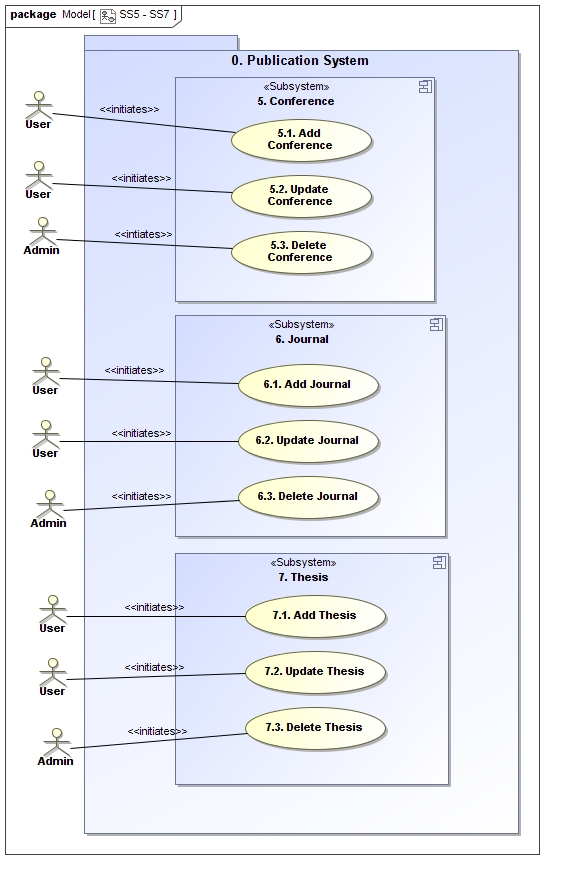
\includegraphics[width=\textwidth]{SS5-SS7}
					\caption{Use case diagram for the Conference, Journal and Thesis Subsystems}
				\end{figure}
			\subsubsection{Report Subsystem}
				\textbf{Pre-Conditions:} User must be logged in to be able to generate a report.\\
				\textbf{Post-Conditions:}
				\begin{itemize}
					\item A simple but comprehensive report must be generated in the format chosen by the user.
					\item The report must only include papers that the current user is associated with.
				\end{itemize}
				
		\subsection{Required Functionality}
			\subsubsection{User Subsystem Use Case}
				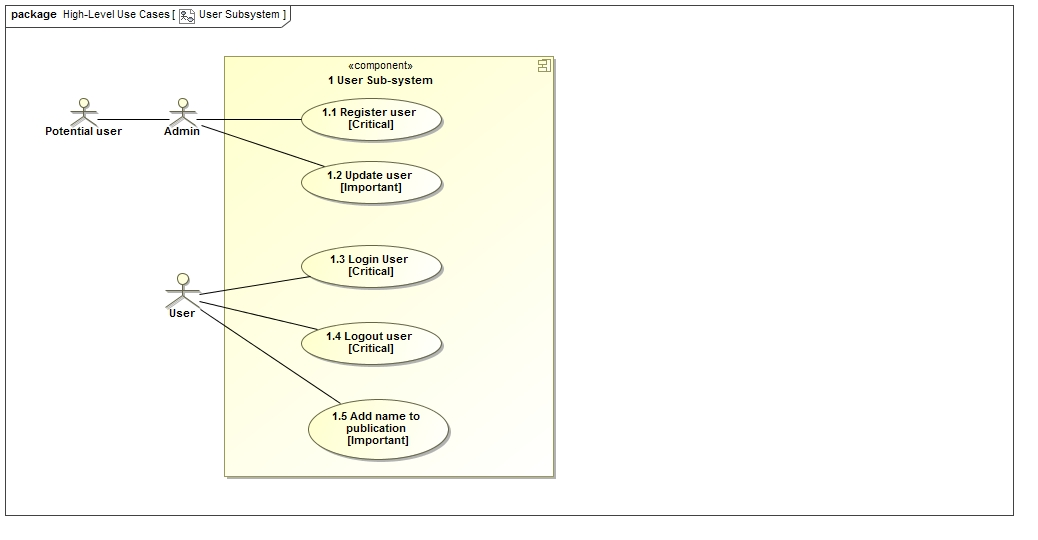
\includegraphics[width=\textwidth]{UserSubsystem}
				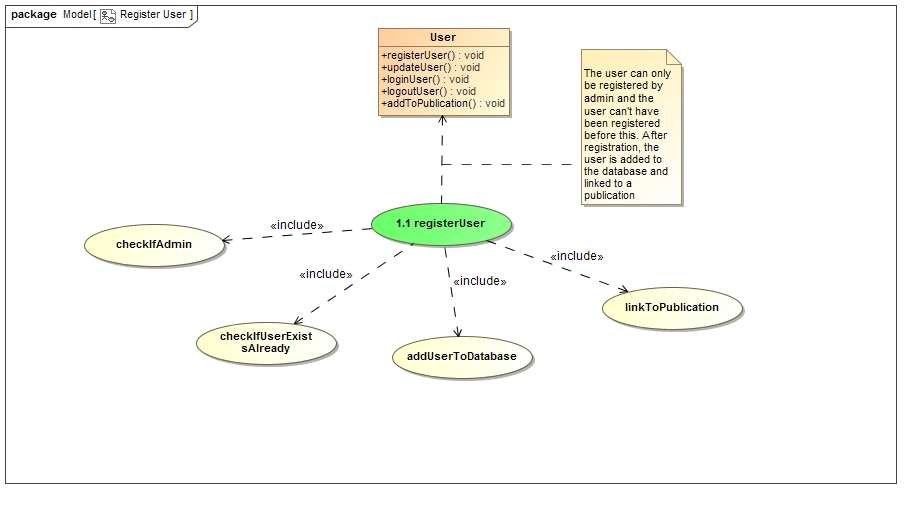
\includegraphics[width=\textwidth]{RegisterUser}
				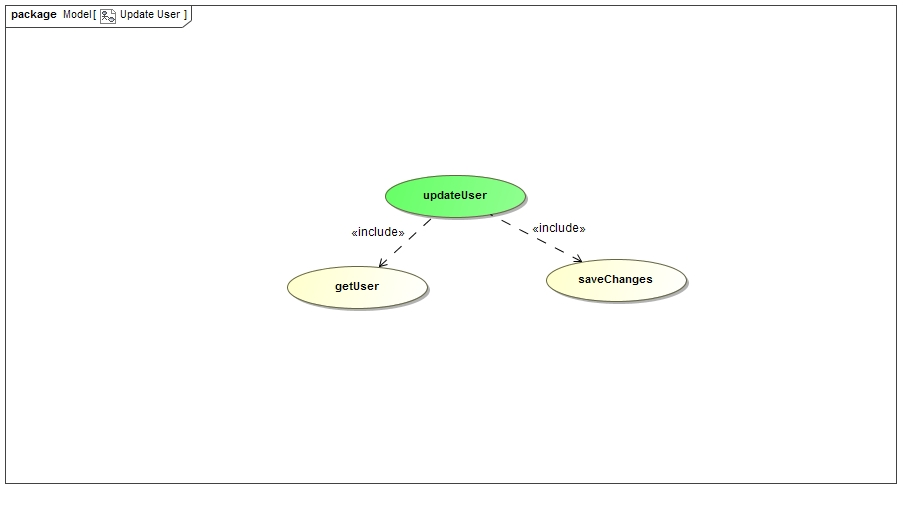
\includegraphics[width=\textwidth]{UpdateUser}
				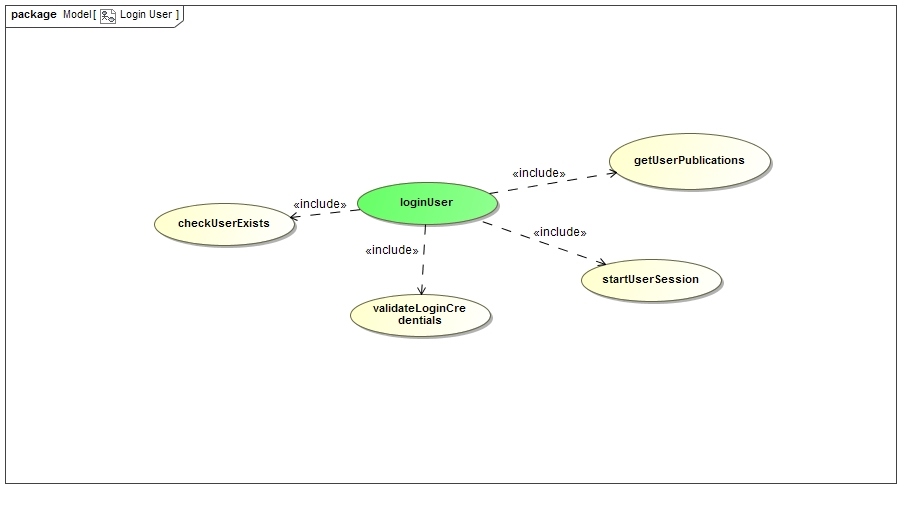
\includegraphics[width=\textwidth]{LoginUser}
				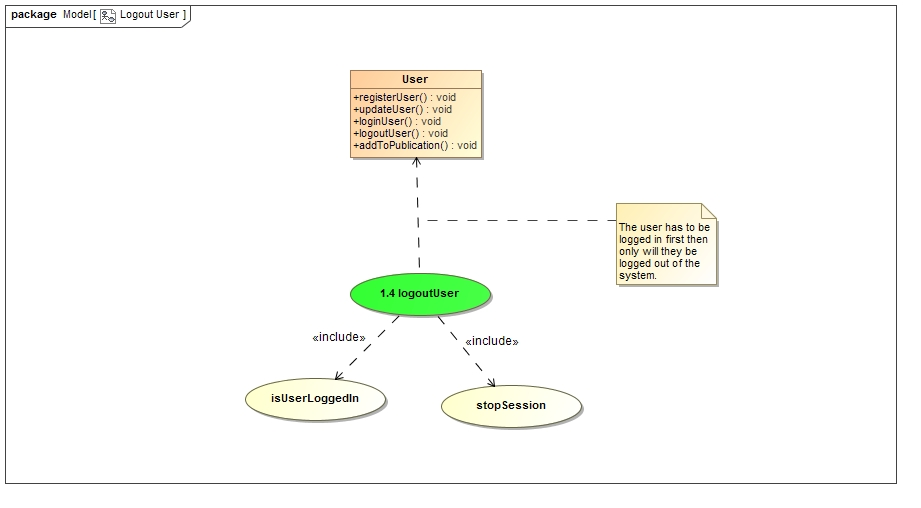
\includegraphics[width=\textwidth]{LogoutUser}
				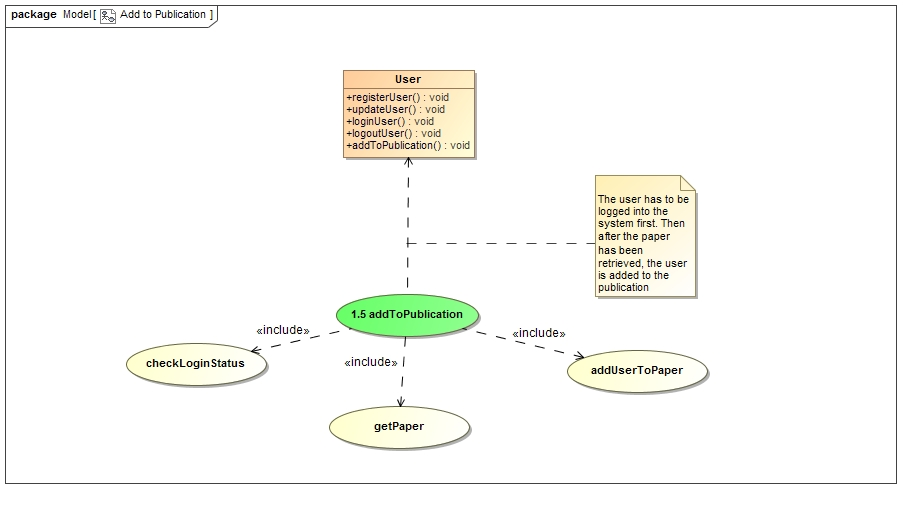
\includegraphics[width=\textwidth]{AddtoPublication}
			\subsubsection{Publication Subsystem Use Case}
				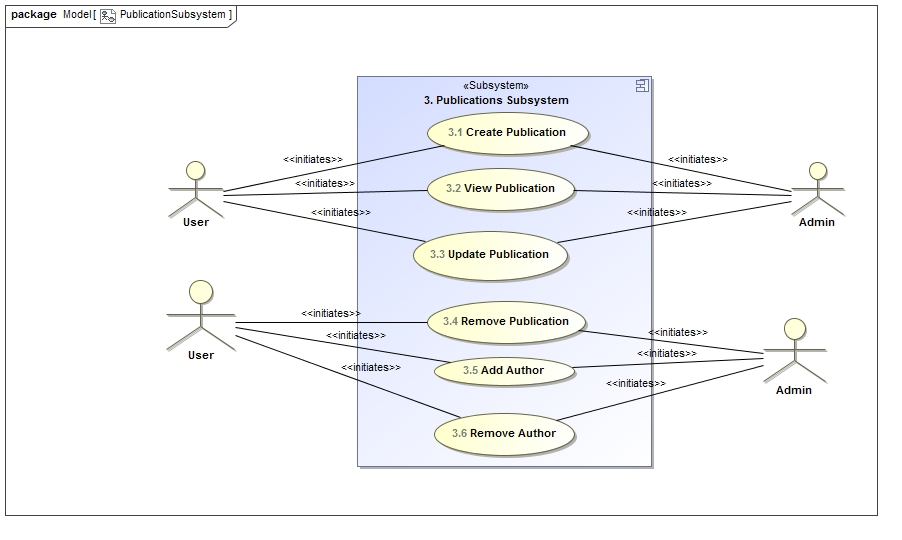
\includegraphics[width=\textwidth]{SS3_PublicationSubsystem}
				\begin{figure}
					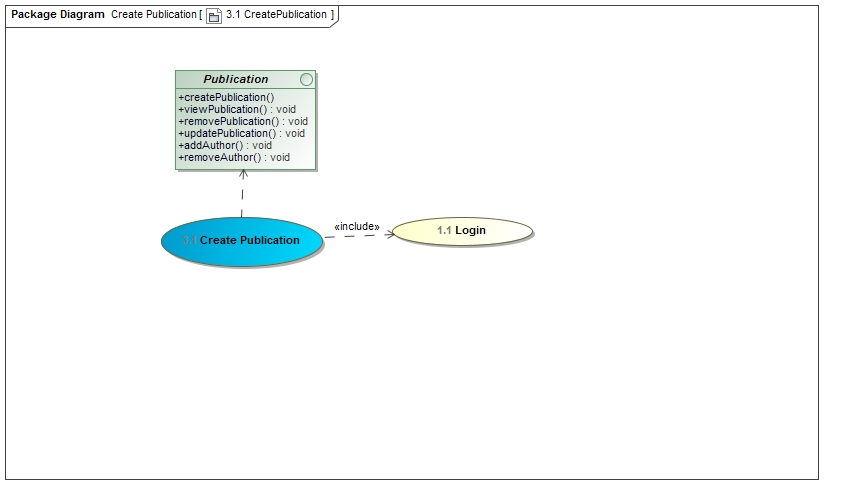
\includegraphics[width=\textwidth]{"5.3 SS3"/SS3-1_CreatePublication}
					\caption{Create Publication}
				\end{figure}
				\begin{figure}
					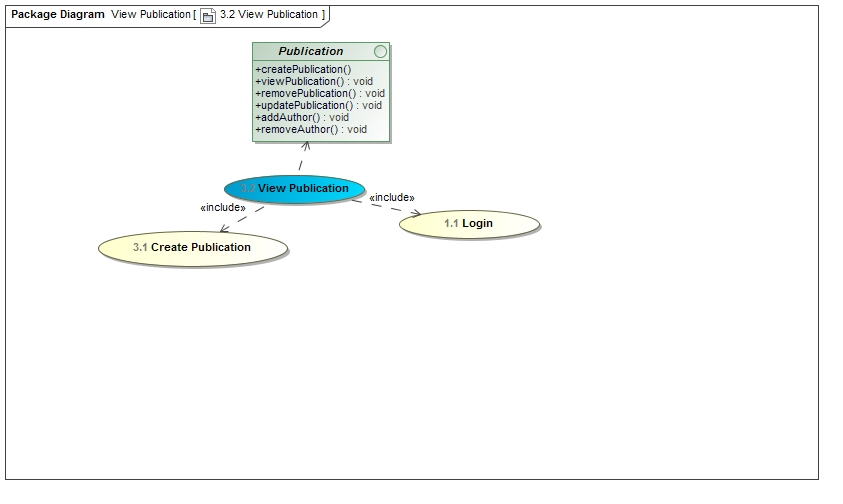
\includegraphics[width=\textwidth]{"5.3 SS3"/SS3-2_ViewPublication}
					\caption{View Publication}
				\end{figure}
				\begin{figure}
					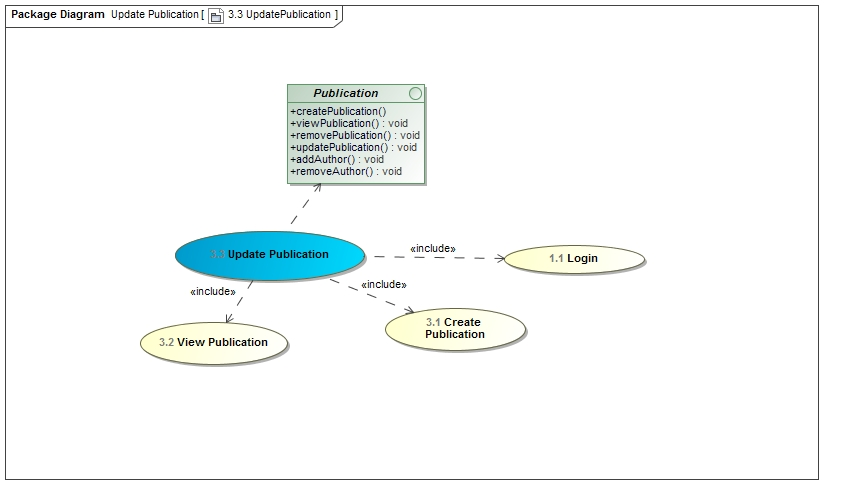
\includegraphics[width=\textwidth]{"5.3 SS3"/SS3-3_UpdatePublication}
					\caption{Update Publication}
				\end{figure}
				\begin{figure}
					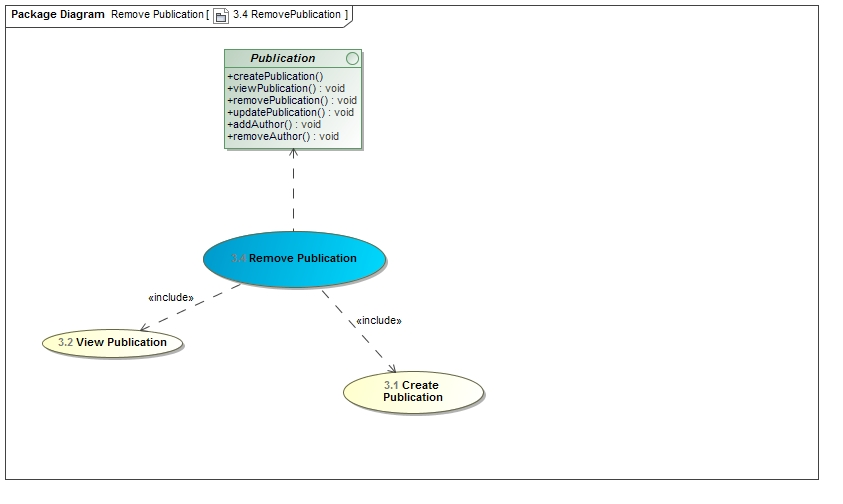
\includegraphics[width=\textwidth]{"5.3 SS3"/SS3-4_RemovePublication}
					\caption{Remove Publication}
				\end{figure}
				\begin{figure}
					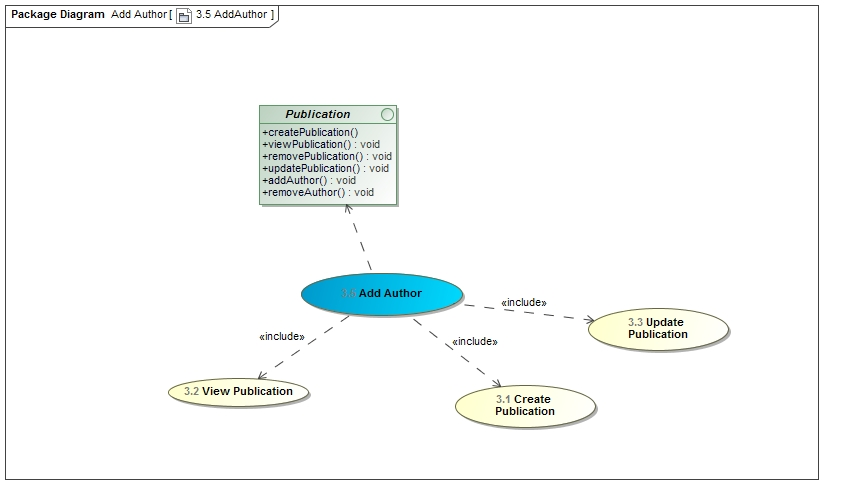
\includegraphics[width=\textwidth]{"5.3 SS3"/SS3-5_AddAuthor}
					\caption{Add Author}
				\end{figure}
				\begin{figure}
					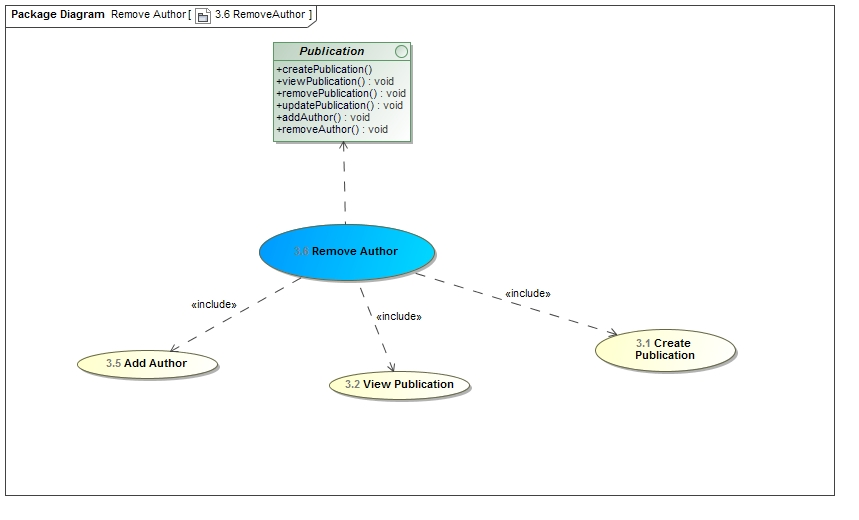
\includegraphics[width=\textwidth]{"5.3 SS3"/SS3-6_RemoveAuthor}
					\caption{Remove Author}
				\end{figure}
			\subsubsection{Research Group Subsystem Use Case}
				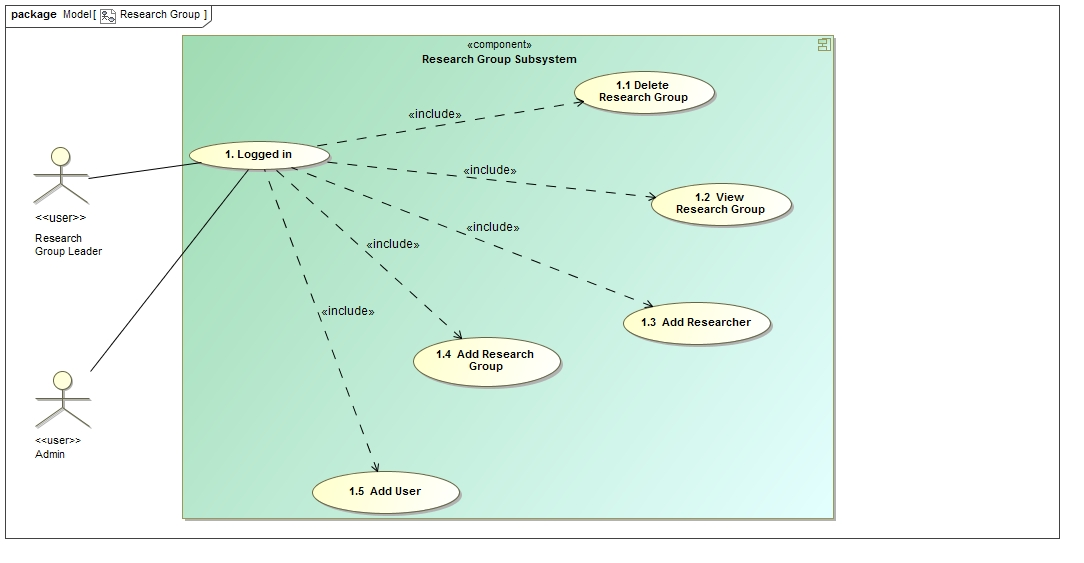
\includegraphics[width=\textwidth]{ResearchGroup}
			\subsubsection{Conference Subsystem Use Case}
				\begin{figure}
					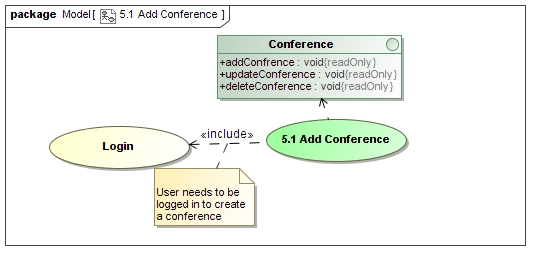
\includegraphics[width=\textwidth]{5.3-SS5-7/Add-Conference}
					\caption{Add Conference}
				\end{figure}
				\begin{figure}
					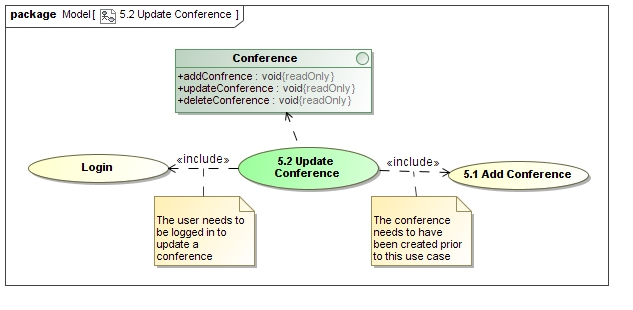
\includegraphics[width=\textwidth]{5.3-SS5-7/Update-Conference}
					\caption{Update Conference}
				\end{figure}
				\begin{figure}
					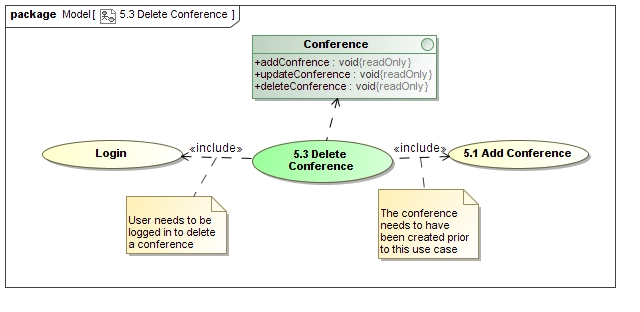
\includegraphics[width=\textwidth]{5.3-SS5-7/Delete-Conference}
					\caption{Delete Conference}
				\end{figure}
			\subsubsection{Research and authors Subsystem Use Case}
				\begin{figure}
					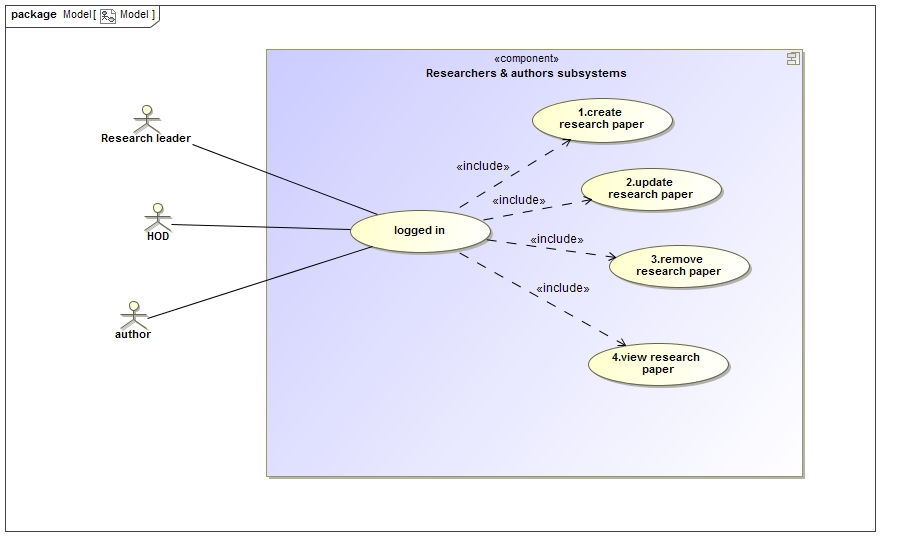
\includegraphics[width=\textwidth]{authorsSubsystem}
					\caption{Research and authors use case diagram}
				\end{figure}
			\subsubsection{Journal Subsystem Use Case}
				\begin{figure}
					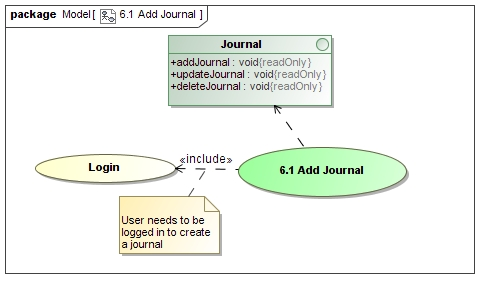
\includegraphics[width=\textwidth]{5.3-SS5-7/Add-Journal}
					\caption{Add Journal}
				\end{figure}
				\begin{figure}
					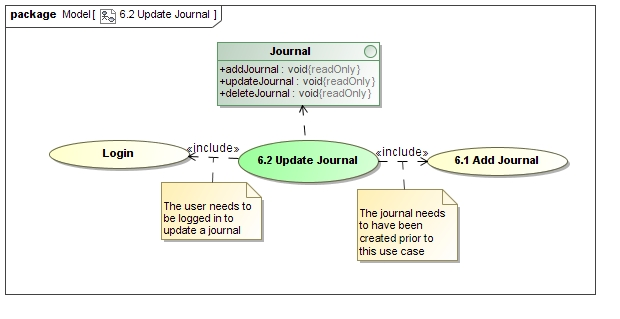
\includegraphics[width=\textwidth]{5.3-SS5-7/Update-Journal}
					\caption{Update Journal}
				\end{figure}
				\begin{figure}
					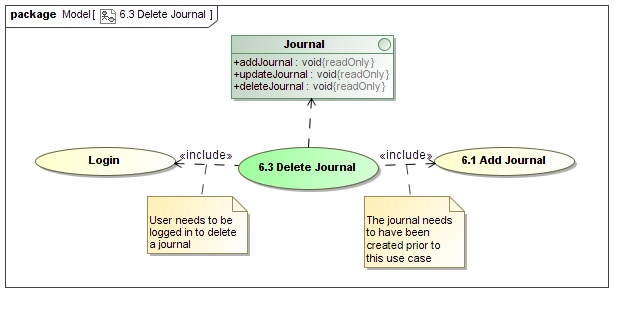
\includegraphics[width=\textwidth]{5.3-SS5-7/Delete-Journal}
					\caption{Delete Journal}
				\end{figure}
			\subsubsection{Thesis Subsystem Use Case}
				\begin{figure}
					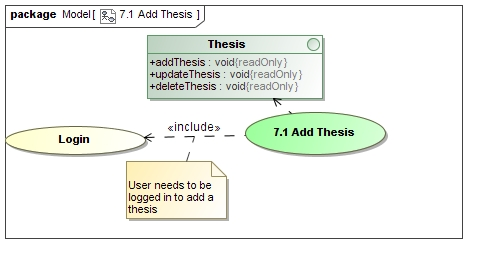
\includegraphics[width=\textwidth]{5.3-SS5-7/Add-Thesis}
					\caption{Add Thesis}
				\end{figure}
				\begin{figure}
					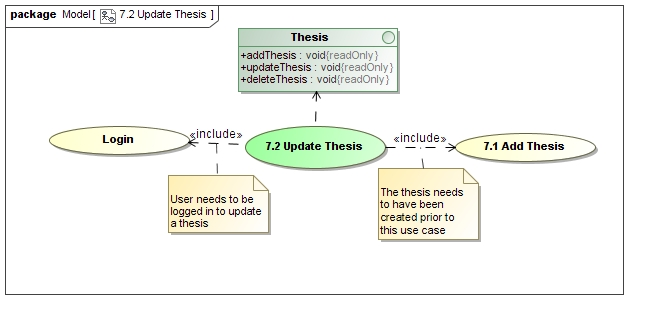
\includegraphics[width=\textwidth]{5.3-SS5-7/Update-Thesis}
					\caption{Update Thesis}
				\end{figure}
				\begin{figure}
					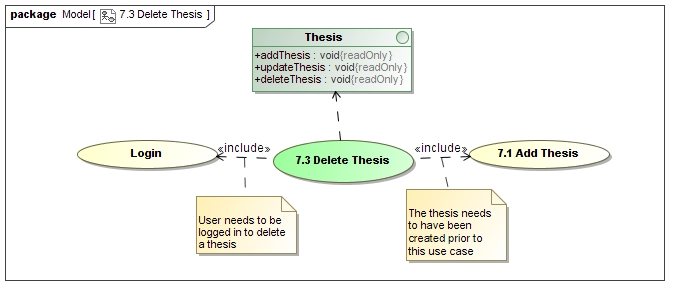
\includegraphics[width=\textwidth]{5.3-SS5-7/Delete-Thesis}
					\caption{Delete Thesis}
				\end{figure}
			\subsubsection{Report Subsystem Use Case}
				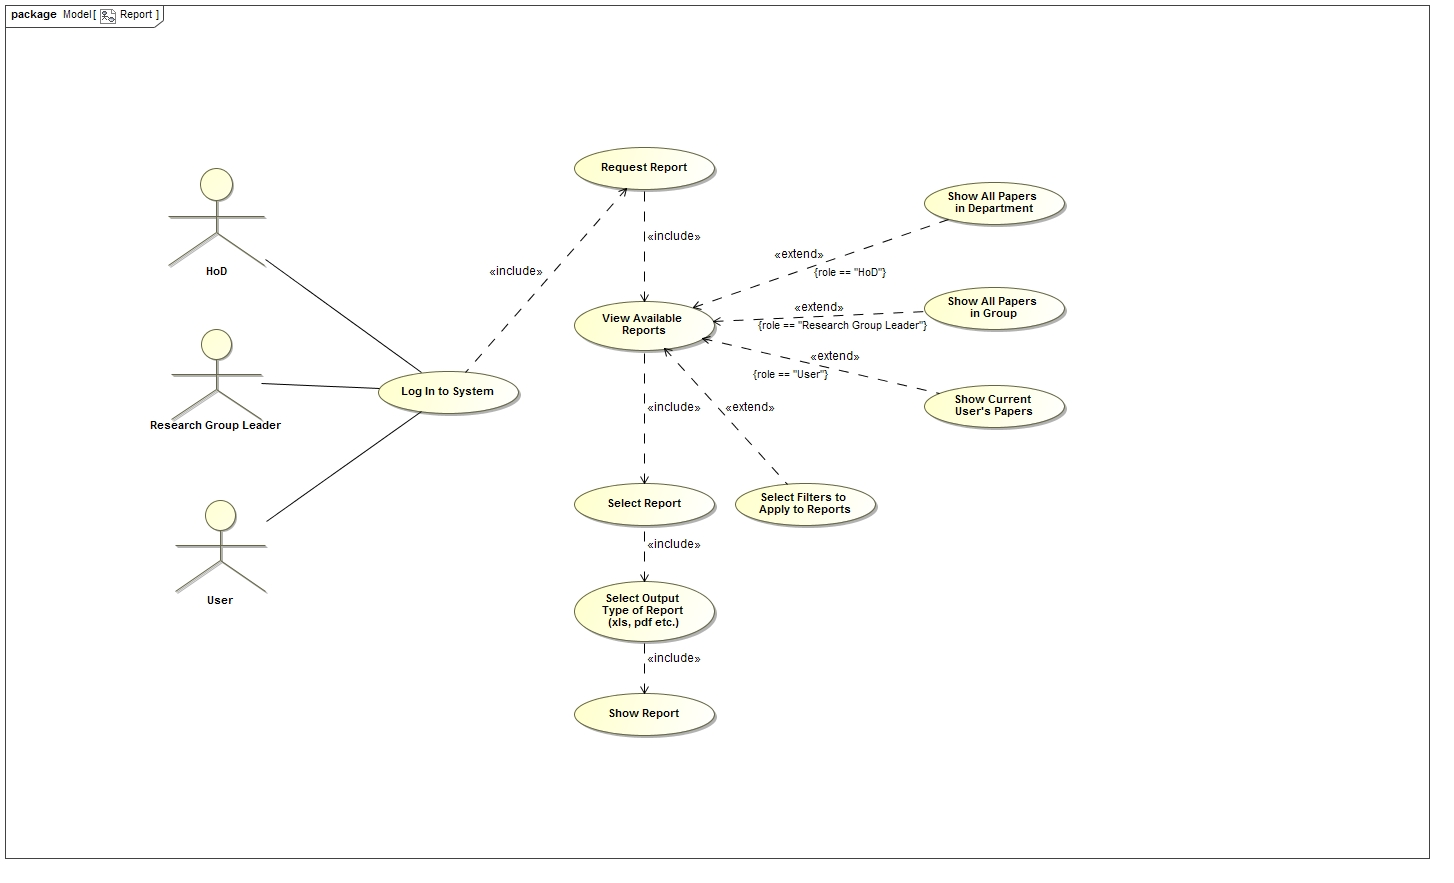
\includegraphics[width=\textwidth]{ReportUseCase}
		\subsection{Process Specifications}
			\subsubsection{Conference Subsystem}
				\begin{figure}[h]
					\centerline{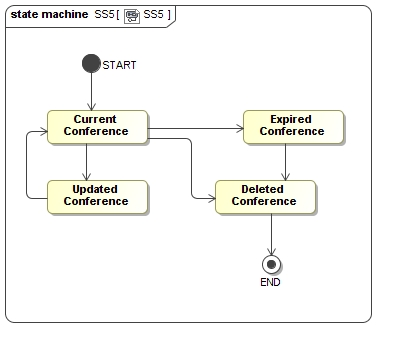
\includegraphics[width=186px]{5.4-SS5-7/SS5}}
					\caption{Conference State Diagram}
				\end{figure}
				\newpage
			\subsubsection{Journal Subsystem}
				\begin{figure}[h]
					\centerline{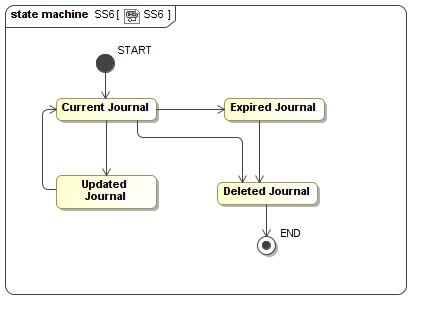
\includegraphics[width=186px]{5.4-SS5-7/SS6}}
					\caption{Journal State Diagram}
				\end{figure}
			\subsubsection{Thesis Subsystem}
				\begin{figure}[h!]
					\centerline{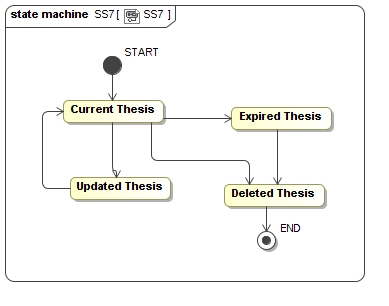
\includegraphics[width=186px]{5.4-SS5-7/SS7}}
					\caption{Thesis State Diagram}
				\end{figure}
				\newpage
		\subsection{Domain Model}
			\begin{figure}[h!]
				\centerline{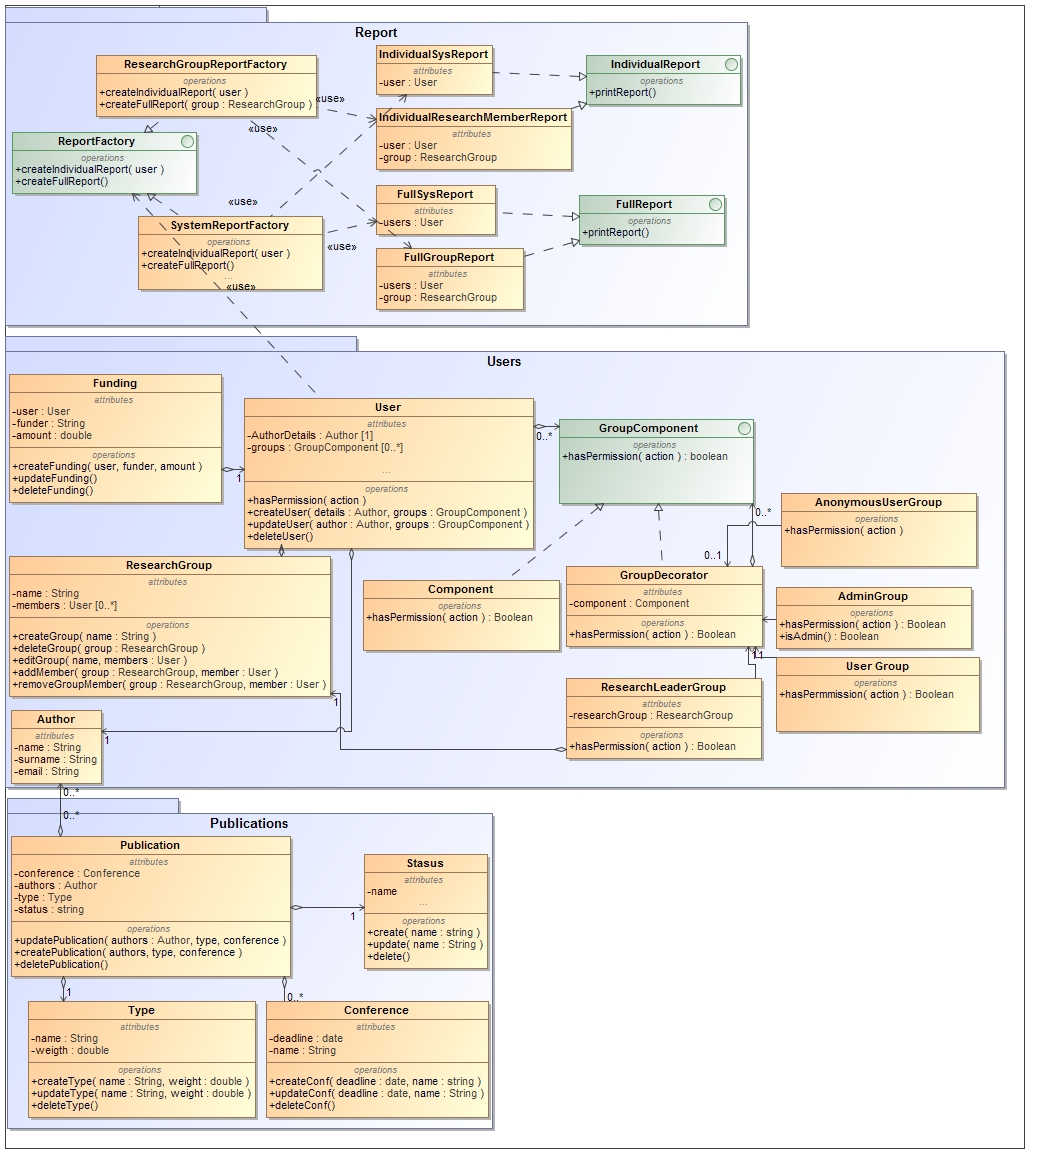
\includegraphics[width=186px]{DomainModel/DomainModel}}
					\caption{Domain Model}
			\end{figure}
	\section{Open Issues}
	\begin{itemize}
		\item Specifics with regard to the DoE and UP weighted contributions
		\item Further elaboration on how funding occurs.
	\end{itemize}
	
	\section{Architectural Tactics or Strategies}
	
	\begin{itemize}
		\item Scalability - It is estimated that there will be approximatly one hundred users. The system should be able to handle each user being active at the same time even though it is unlikly.
	\end{itemize}
		\subsection{Reliability}
			Any data that is added to the system must be checked before it is stored. Any incorrect data (e.g. letters in a date) must be fixed before the form can be submitted. This ensures that the stored information is consistent.\\
			
			A strict format must be applied to any reporting and any generated report must follow the format. If needed data is missing, there should be stand-in messages (such as "No data available").
		\subsection{Scalability}
			In order to reduce the load of multiple users, use cases that are common (such as some reports) should be optimized.\\
			
			If multiple users have access to the same resources, the addition of data should be done on a first-come-first-serve basis, and the newest information should override older data.\\
			
			When the amount of users logged in exceeds the load capabilities of the server, the server should be able to scale up in order to handel the excess requests.
		\subsection{Cost}
			Reports could be pre-processed and cached so that the same report is not generated multiple times, saving on resources. The system should be able to produce subsets of the report at a relativly low cost (e.g. a report for all researchers under a specific research group), and re-use those subsets to make the larger reports.
		\subsection{Security}
			Strict user control must be enforced, ensuring that each step of any use case makes sure that the user has the correct authorisation. By using hashing, passwords can be stored safely in the database, with a lower risk to user information leaks. \textbf{No plaintext passwords should be stored}.
		\subsection{Audibility}
			By using multiple log files, the different kinds of actions can be individually logged (i.e. individual logs for Errors, Logins, Data changes etc.), and there should be log files for individual days (a new log for each day) so that the information is organised. Over time, old log files can be merged together for archiving purposes.

\end{document}
